\documentclass[12pt]{article}
\usepackage{sbc-template}
\usepackage{graphicx,url}
\usepackage[brazil]{babel}   
\usepackage[latin1,utf8]{inputenc}  
\documentclass[a4paper,11pt]{book}
\graphicspath{{img/}}

\sloppy

\title{Projeto de Engenharia de Software \\ UP! SHARING}

\address{Instituto de Informática - Instituto de Pesquisas Tecnologicas do Estado de São Paulo (IPT)\\ Caixa Postal 15.064 - 91.501-970 -- São Paulo -- SP -- Brazil}

\author{Alex A. Prado\inst{1}, Dirce Mudrai\inst{1}, Ivan Borges\inst{1} \email{alex.azprado@gmail.com, dirce.mudrai@icloud.com,
  ivangb@gmail.com}}


\begin{document} 

\maketitle

\begin{abstract}


  This meta-paper describes the style to be used in articles and short papers
  for SBC conferences. For papers in English, you should add just an abstract
  while for the papers in Portuguese, we also ask for an abstract in
  Portuguese (``resumo''). In both cases, abstracts should not have more than
  10 lines and must be in the first page of the paper.
  
 
\end{abstract}
     
\begin{resumo} 
  Este meta-artigo descreve o estilo a ser usado na confec��o de artigos e
  resumos de artigos para publica��o nos anais das confer�ncias organizadas
  pela SBC. � solicitada a escrita de resumo e abstract apenas para os artigos
  escritos em portugu�s. Artigos em ingl�s dever�o apresentar apenas abstract.
  Nos dois casos, o autor deve tomar cuidado para que o resumo (e o abstract)
  n�o ultrapassem 10 linhas cada, sendo que ambos devem estar na primeira
  p�gina do artigo.
\end{resumo}


\section{Introdução ao Projeto}

Esse projeto de engenharia de software, que estará disponível para dispositivos móveis, com acesso à infraestrutura em nuvem. Visa suprir uma necessidade da montadora em fornecer serviço de locação para uma linha específica de veículos, muito usada em locação de modo compartilhado. Este tipo de locação possibilita diversos ganhos econômicos, sociais e ambientais.

Entende-se locação compartilhada (CAR SHARING) como a forma de utilização comunitária de um mesmo veículo como meio de transporte dada a sua disponibilidade. Este termo é utilizado para definir um modelo de aluguel de veículos em que o cliente aluga o carro para uma quantidade específica ou para uso rápido, com um conceito de autos serviço, em que o cliente é independente e autônomo na utilização do serviço.


\section{Requisitos de Software}
\section{Design de Software}
\section{Construção de Software}
\section{Teste de Software}
\section{Manutenção de Software}
\section{Gerenciamento de Configuração de Software}
\section{Gerenciamento da Engenharia de Software}
\section{Processo da Engenharia de Software}


\section{Modelos e Métodos na Engenharia de Software}

O projeto UP! Sharing, será desenvolvido de maneira organizada e sistemática para garantir a entrega do produto final utilizando os métodos e ferramentas de engenharia de software adequados. 
As ferramentas da engenharia de software fornecem suporte automatizado ou semiautomatizado para o processo e para os métodos. Quando as ferramentas são integradas, de modo que as informações criadas por uma ferramenta possam ser utilizadas por outra, é estabelecido um sistema para o suporte ao desenvolvimento de software.
\cite{pressman2016engenharia}

Os métodos da engenharia de software fornecem as informações técnicas para desenvolver software. Os métodos envolvem uma ampla variedade de tarefas, que incluem: comunicação, análise de requisitos, modelagem de projeto, construção de programa, testes e suporte. Os métodos da engenharia de software se baseiam em um conjunto de princípios básicos que governam cada área da tecnologia e incluem atividades de modelagem e outras técnicas descritivas.

O método ágil para gestão de projetos apresenta um modelo mais amigável de gestão que outros por este motivo, foi definido como sendo mais adequado para o projeto. O scrum master gerencia as atividades de maneira incremental que recebe o nome de Sprint e não pode durar mais de 30 dias. A lista do Product Backlog Item (PBI) é gerada a partir das atividades que são identificadas, definidas, priorizadas e estimadas. Uma versão funcional do software é testada e liberada em cada incremento. As reuniões diárias Daily Scrum meentings garante que o trabalho esteja de acordo com o plano. \cite{Bourque2014}

\begin{figure}[htp]
\centering
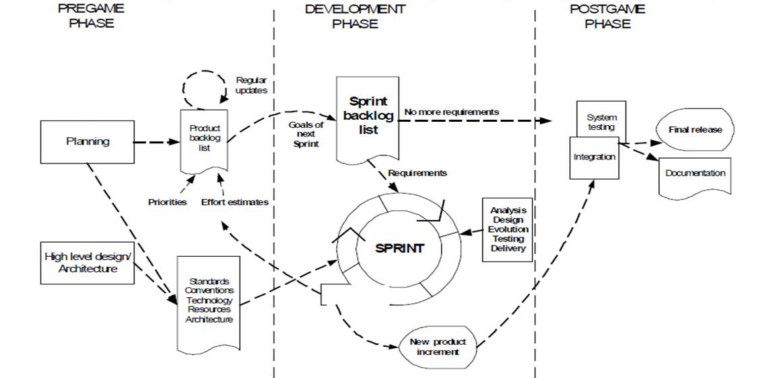
\includegraphics[width=.9\textwidth]{ScrumModel.png}
\caption{O Scrum como mostrado na figura acima é um quadro de gerenciamento de projetos de propósito geral que é aplicável a qualquer projeto com prazos agressivos com requisitos complexos e um grau de singularidade \cite{rees2002feasible}}
\label{fig:exampleFig3}
\end{figure}

O termo Scrum originalmente deriva de uma estratégia no jogo de rugby onde denota "obter uma bola fora de jogo de volta para o jogo" com o trabalho em equipe. O Scrum depende do auto-empenho, da auto-organização e da emergência em vez de medidas autoritárias. O Scrum é adequado para pequenas equipes de menos de 10 engenheiros. O processo Scrum inclui 3 fases: pré-jogo, desenvolvimento e pós-jogo.

A \textbf{fase pré-jogo} inclui 2 subfases:
    
Planejamento: inclui a definição do sistema que está sendo desenvolvido. É criada uma lista de backlog de produtos contendo todos os requisitos conhecidos.

Arquitetura: o design de alto nível do sistema, incluindo a arquitetura, é planejada com base nos itens atuais no Product Backlog.
    
Na \textbf{fase de desenvolvimento}, o sistema é desenvolvido em Sprints que são ciclos iterativos onde a funcionalidade é desenvolvida ou aprimorada para produzir novos incrementos. Cada Sprint inclui: Requisitos, Análise, Design, Evolução e fases de entrega.

A \textbf{fase pós-jogo} contém o encerramento do lançamento, incluindo tarefas como integração, testes de sistema e documentação. \cite{Kumar2014}


\section{Qualidade de Software}

Segundo a norma ISO 9000 (versão 2000), qualidade é "o grau em que um conjunto de características inerentes a um produto, processo ou sistema e cumpre os requisitos inicialmente estipulados para estes". Já \cite{Juran1998}, tem duas definições para qualidade "a característica dos produtos que atendem as necessidades dos clientes, e, assim, proporcionar a satisfação do mesmo" e "qualidade é a ausência de deficiências"

A definição específica sobre qualidade de software mais difundida é a encontrada nas normas ISO/EIC 9126-1 e ISO/IEC 25010, para as quais qualidade é "a capacidade do produto de software em satisfazer as necessidades implícitas e explícitas quando usado em condições específicas".





\section{Práticas Engenharia de Software}
\section{Economia na Engenharia de Software}


\begin{figure}[htp]
\centering
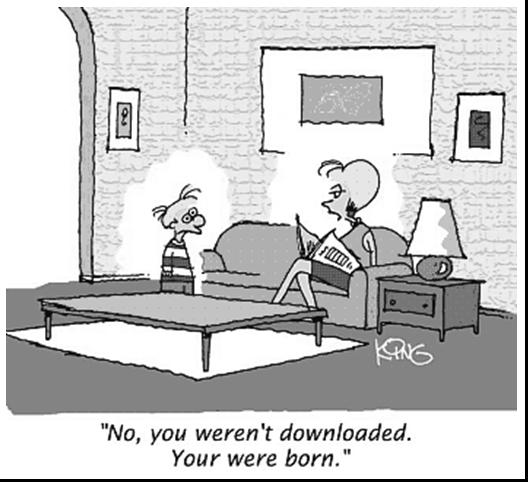
\includegraphics[width=.5\textwidth]{fig1.jpg}
\caption{A typical figure}
\label{fig:exampleFig1}
\end{figure}

\begin{figure}[htp]
\centering
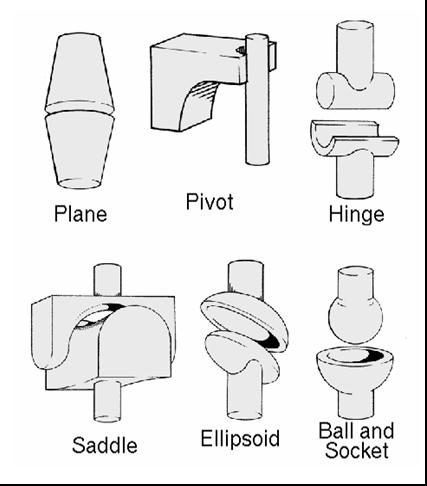
\includegraphics[width=.3\textwidth]{fig2.jpg}
\caption{This figure is an example of a figure caption taking more than one
  line and justified considering margins mentioned in Section~\ref{sec:figs}}
\label{fig:exampleFig2}
\end{figure}

In tables, try to avoid the use of colored or shaded backgrounds, and avoid
thick, doubled, or unnecessary framing lines. When reporting empirical data,
do not use more decimal digits than warranted by their precision and
reproducibility. Table caption must be placed before the table (see Table 1)
and the font used must also be Helvetica, 10 point, boldface, with 6 points of
space before and after each caption.

\begin{table}[ht]
\centering
\caption{Variables to be considered on the evaluation of interaction
  techniques}
\label{tab:exTable1}
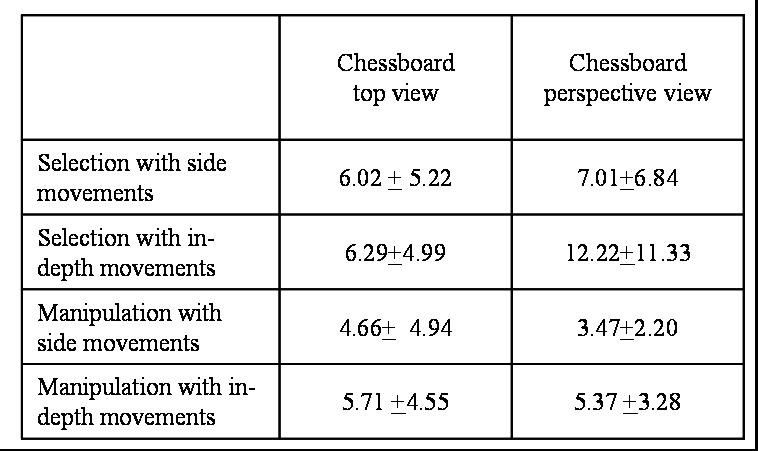
\includegraphics[width=.7\textwidth]{table.jpg}
\end{table}


\section{References}

Bibliographic references must be unambiguous and uniform.  We recommend giving
the author names references in brackets, e.g. \cite{knuth:84},
\cite{boulic:91}, and \cite{smith:99}.

The references must be listed using 12 point font size, with 6 points of space
before each reference. The first line of each reference should not be
indented, while the subsequent should be indented by 0.5 cm.


\bibliographystyle{sbc}
\bibliography{sbc-template}

\end{document}
